\documentclass[12pt]{article}
\usepackage[margin=0.5in]{geometry}
%\documentclass[11pt,preprint]{aastex}
\usepackage{amsmath,amssymb}
\usepackage{natbib}
\usepackage{graphicx} 
\usepackage{setspace}
\usepackage[usenames]{color}
\definecolor{Red}{rgb}{1.00,0.00,0.00}

\newcommand{\degr}{\ensuremath{^\circ}}

\begin{document}
\textbf{PI:} D. J. Schlegel \textbf{Title:} Mass Mapping Abell 2261 with Kinematic Weak Lensing \textbf{ID:} 2014A\_U051D

\section{Science Justification}


\subsection{Cluster Mass Mapping}

The mass distribution in galaxy clusters is a crucial test of our cosmological paradigm. Total halo masses probe the amplitude of matter fluctuations and growth of structure in the Universe, and the abundance of substructure within halos is sensitive to the history of hierarchical assembly and potentially the interaction cross section of dark matter \citep[e.g.,][]{Natarajan2002a, Natarajan2002b, Voit2005, Clowe2006}. Gravitational lensing has played an important role in mapping dark matter within halos, primarily by exploiting the distortion of images of background galaxies. On small scales inside lensing clusters, strong distortions produce extended arcs and multiple images enabling the production of detailed mass maps, while on larger scales the distortions are weaker and require averaging the shapes of many background galaxies over a broad area to extract a shear signal.

We propose to map the projected mass distribution in the massive cluster Abell 2261 with a new lensing techinque that uses kinematic measurements of background sources to drastically improve the signal-to-noise (${\rm S/N}$) per galaxy. The typical weak lensing shear signal averaged within the virial radius of a massive cluster ($\gamma_t\sim0.05$) is small compared to the distribution of intrinsic shapes in imaging (which has scatter $\sigma_\gamma\sim0.25$). Kinematic information can be used to infer the intrinsic shape and orientation of the background galaxies, potentially reducing the shape noise per galaxy by a factor of ten. This enables ${\rm S/N}\gtrsim1$ measurements of shear with individual galaxies. With such precision we will improve the spatial resolution of mass maps and extend the precision of strong lensing out to the weak regime near the virial radius of the cluster. We discuss this technique and its potential for improving both the precision and accuracy of future large-scale lensing experiments in the next section. Additionally, the repeat slit spectra taken for hundreds of sources behind A2261 will provide two-dimensional kinematics of emission line disk galaxies, greatly enhancing the sample size at that redshift for studying evolution of galaxy kinematics and the Tully-Fisher relation (TFR).

\begin{figure}[t]
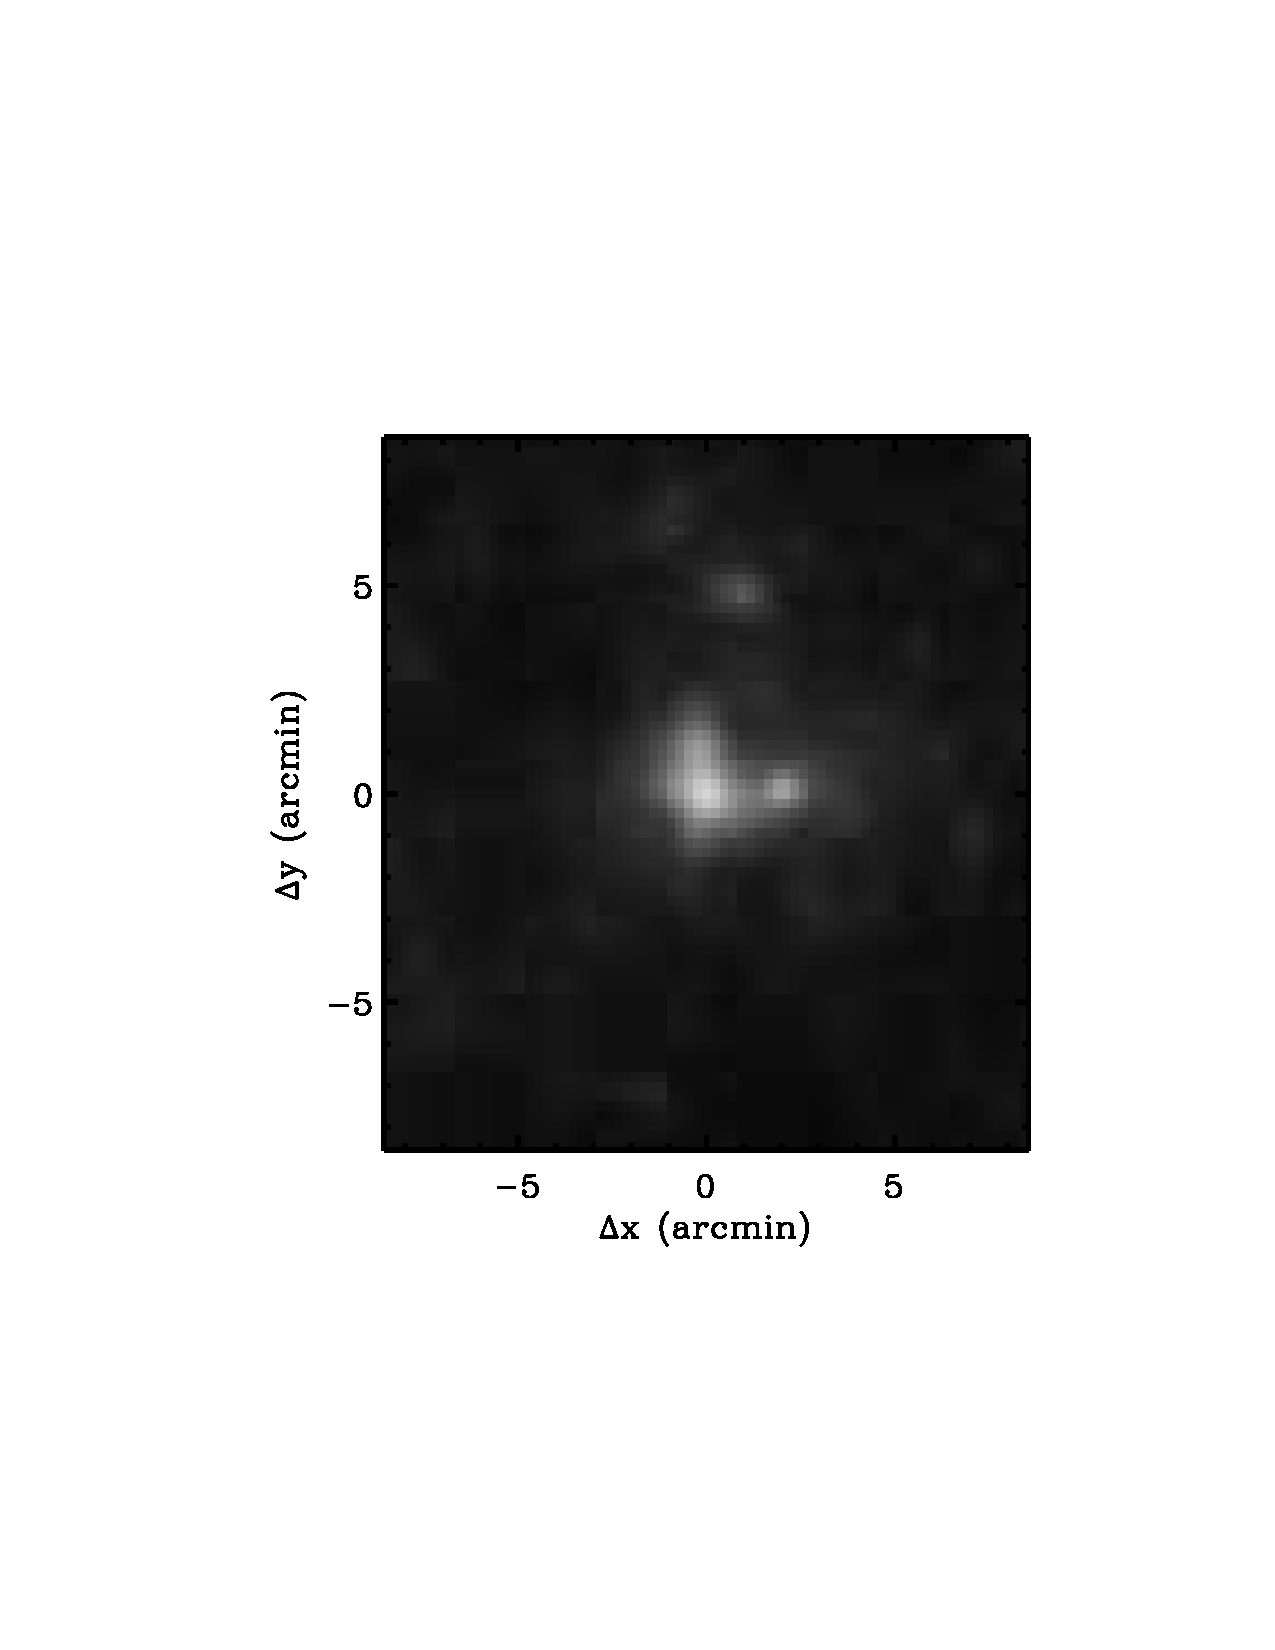
\includegraphics[width=0.3\linewidth,bb= 160 150 500 650,clip]{Plots/shear_map_kappa.pdf}
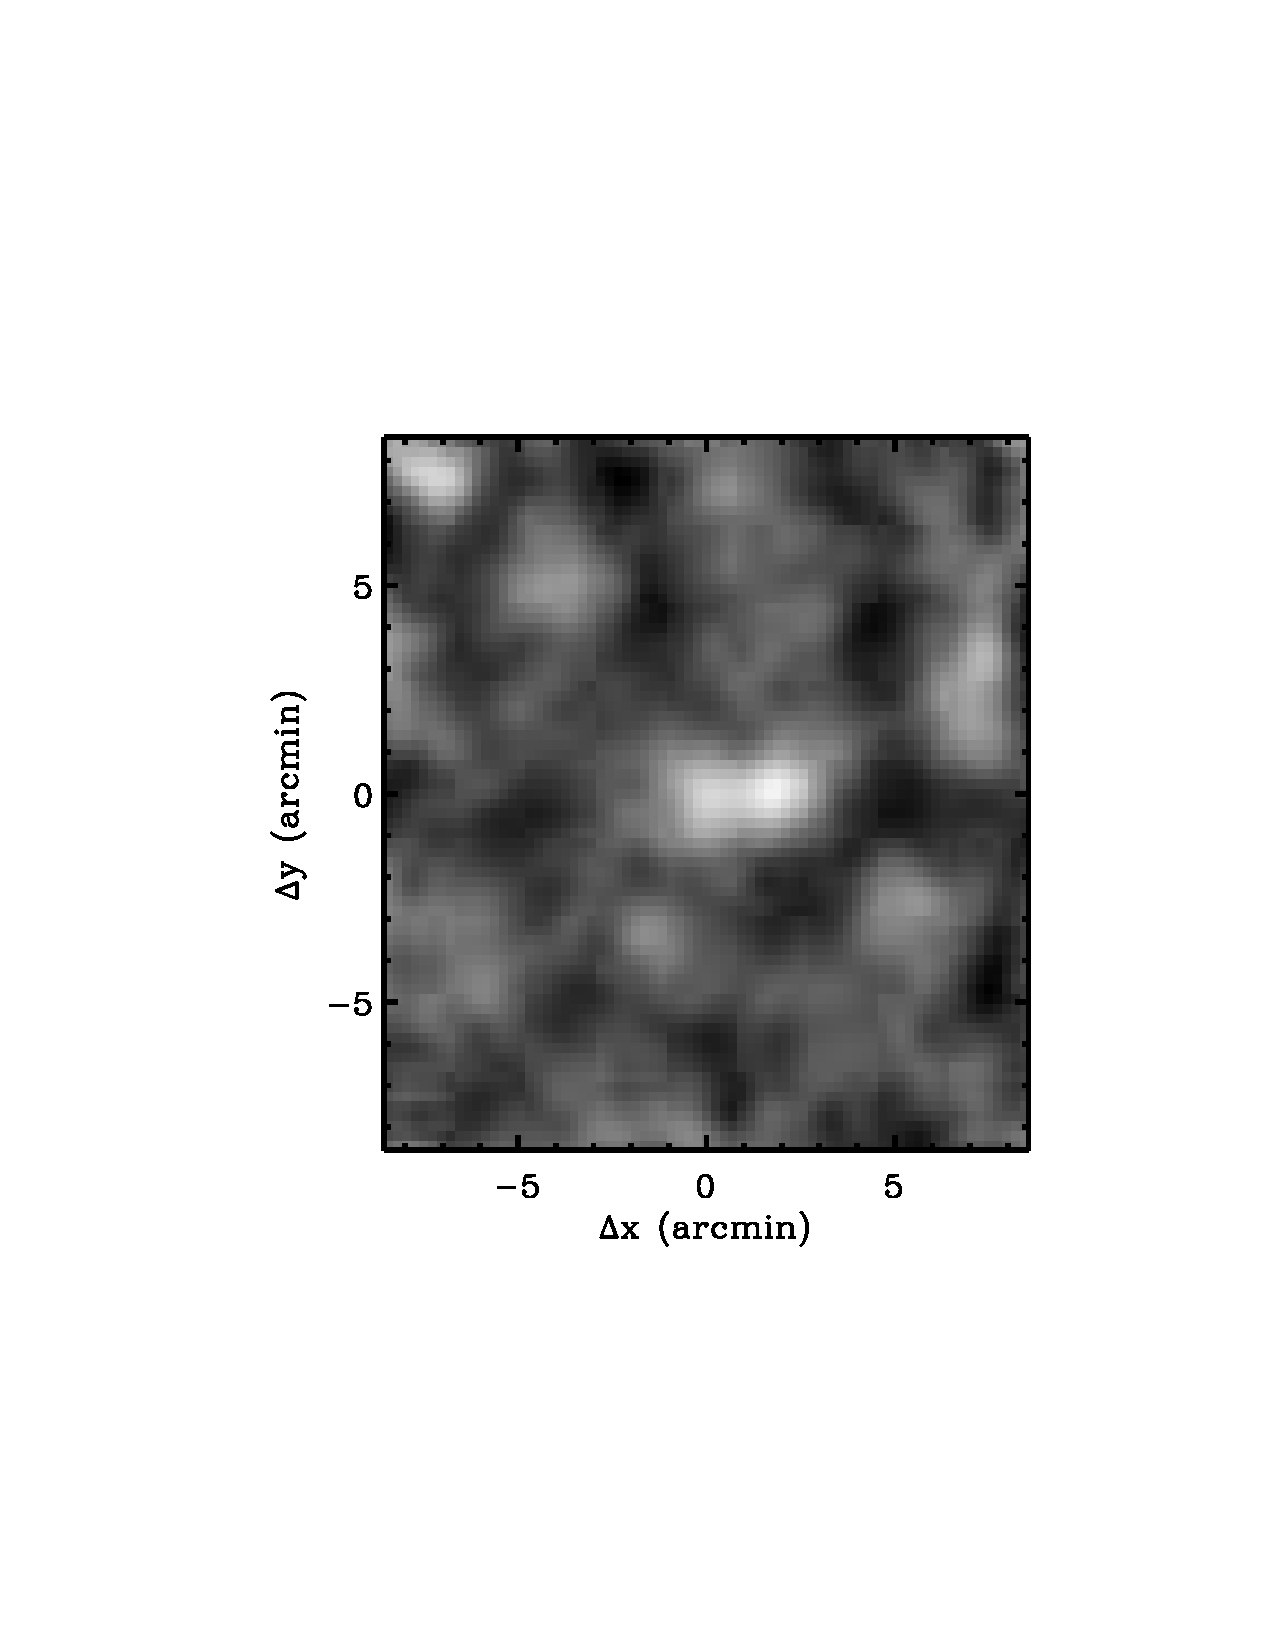
\includegraphics[width=0.3\linewidth,bb= 160 150 500 650,clip]{Plots/shear_map_subaru.pdf}
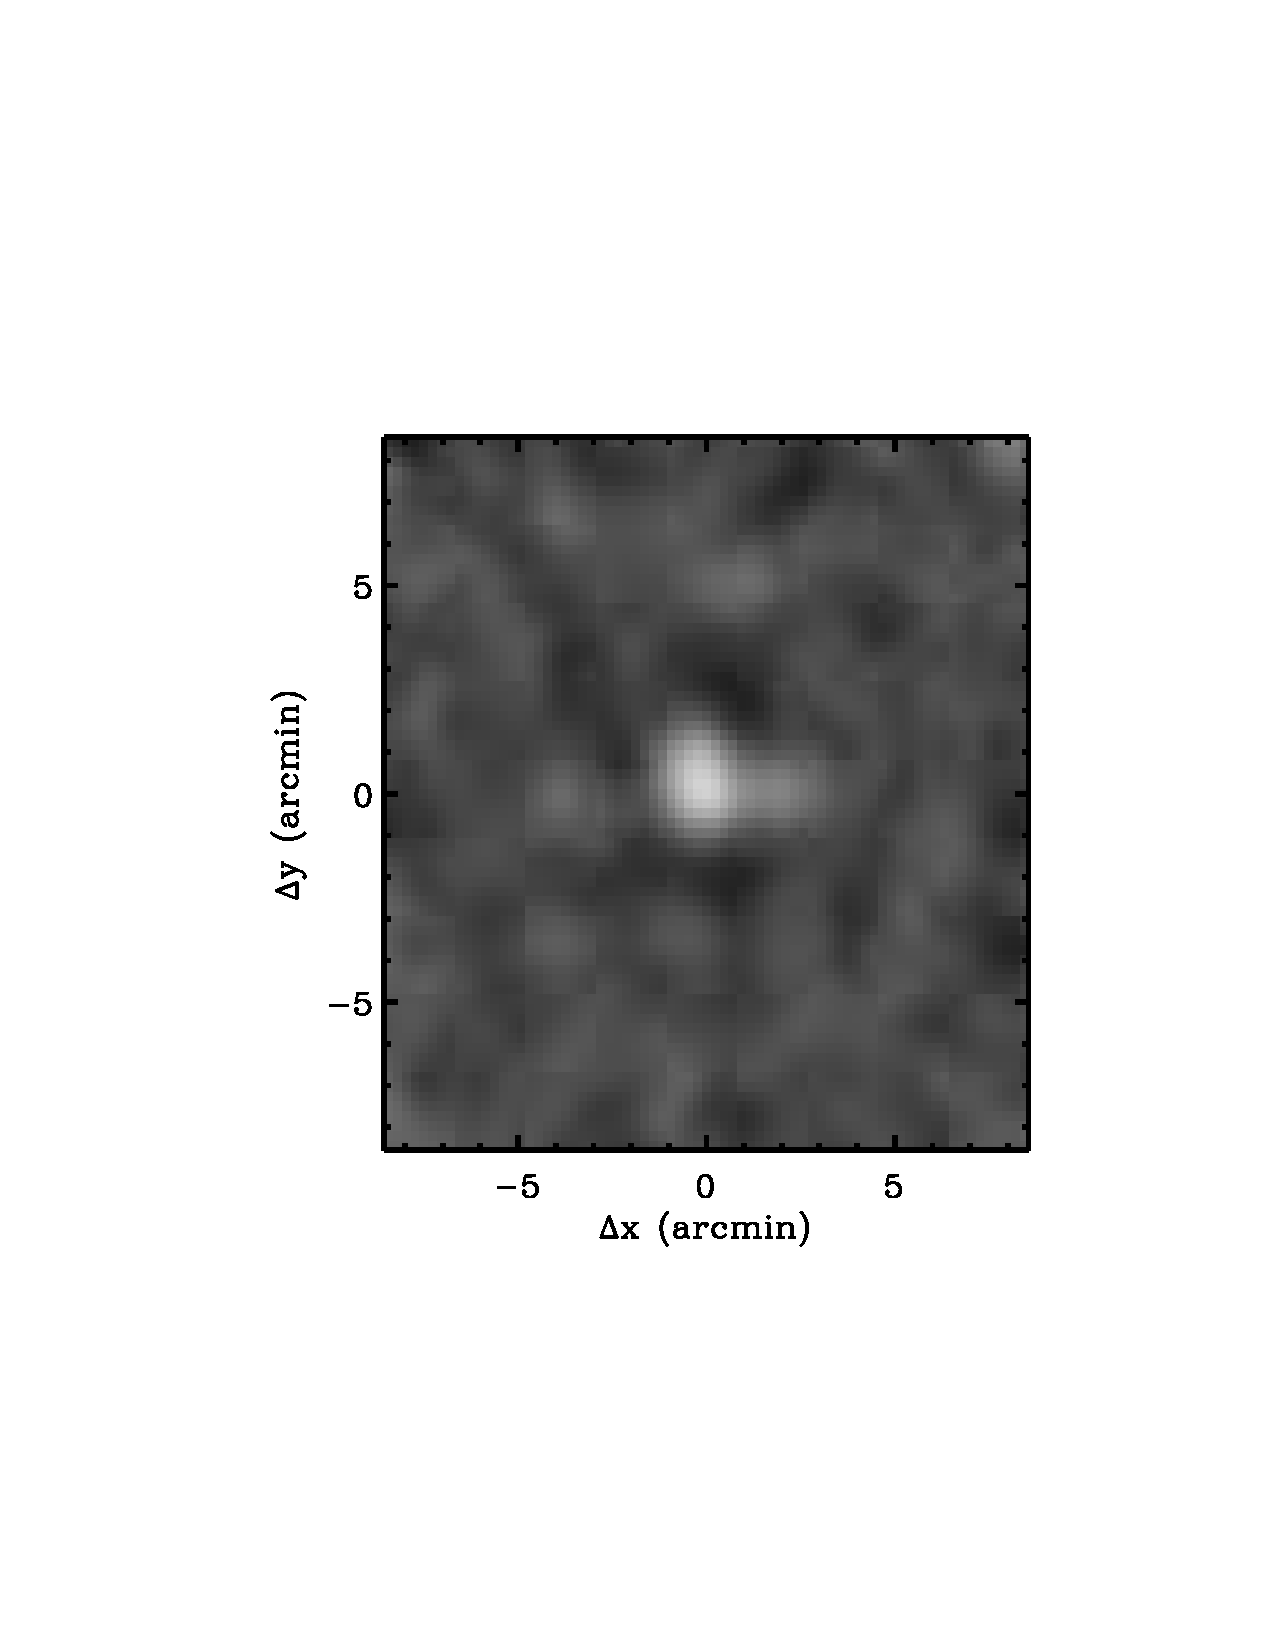
\includegraphics[width=0.3\linewidth,bb= 160 150 500 650,clip]{Plots/shear_map_tf.pdf}
\caption{\footnotesize {\bf Left:} mass map, from \citet{Vale2003} simulations, zoomed in on a distended $~10^{15}M_{\odot}$ cluster. {\bf Center:} Aperture mass map with shape noise properties equivalent to existing Subaru observations of A2261. {\bf Right:} Aperture mass map with shape noise properties equivalent to proposed TFR lensing survey. In both cases, we used a compensated aperture mass filter as in \citet{Schneider1998} with $\ell=1$ and the filter scale set to $3$ arcminutes. Peak values in both mass maps are at $\kappa=.08$}
\label{fig:massmaps}
\end{figure}

\subsection{Kinematic Weak Lensing}

The utility of kinematic maps for weak lensing was originally described by \citet{Blain2002} and \citet{Morales2006}, who forecasted constraints from high ${\rm S/N}$, high spatial resolution observations with future radio arrays. The basic idea for the kinematic shear observables is described in Figure~1 of \citet{Morales2006}. In an image, an inclined rotating circular disk has elliptical isophotes. When the image of this galaxy is sheared, the isophotes remain elliptical (in the weak shear limit, $|\gamma_t|\ll1$) with a new axis ratio and position angle. New photometric axes are inferred from this ellipse in the sheared image, and information about the original axes is lost. The case is different however, with kinematic measurements. The unsheared circular disk has kinematic axes that are perpendicular to one another and are aligned with the unsheared photometric axes. This cross shape becomes skewed when the velocity map is sheared; the kinematic axes are no longer perpendicular and they are misaligned with the photometric axes inferred from the sheared isophotal ellipse in the imaging data.

Full two-dimensional kinematic maps are not required for this measurement, and our approach adds to the previous discussion by incorporating information from the TFR, an empirical scaling relation for disk galaxies between their luminosity and circular velocity $v_{\rm circ}$. With slit spectroscopy, the measured amplitude of a rotation curve is related to the true circular velocity by $v_{\rm obs} = v_{\rm circ} \sin i$, where $i$ is the inclination of the disk toward the observer. Thus the offset between $v_{\rm obs}$ and $v_{\rm circ}$ predicted from the TFR gives a kinematic estimate of $\sin i$. Typically observers estimate $\sin i$ from the ellipticity of the image. The difference between the photometric and kinematic estimates of $\sin i$ gives an estimate of the shear.

For ideal circular disks, the shear can be measured to arbitrary precision, limited only by the spatial and spectral resolution of the data. In practice, the precision of the shear measurement is limited by the intrinsic scatter of the TFR, which arises from effects including disk noncircularity, bulges, warps, and winds. After inclination correction, estimates for the intrinsic fractional scatter in $v_{\rm circ}$ at fixed luminosity or stellar mass are typically $0.05-0.06\,{\rm dex}$ both locally and to $z\sim1.3$ \citep{Reyes2011, Miller2011}. For a properly weighted estimator of the galaxy shape based on the TFR offset, this scatter maps to an uncertainty in the intrinsic galaxy ellipticity of only $\sigma_{\epsilon, {\rm TFR}}=0.015$. This should be compared to the intrinsic shape noise for pure disks $\sigma_{\epsilon, {\rm disks}}=0.59$ and for real imaging surveys $\sigma_{\epsilon, {\rm im}}\approx0.4$, and is related to the shear noise through $\sigma_\epsilon / \sigma_\gamma \approx 2(1-\sigma_\epsilon^2)$\citep{Bernstein2002, Hirata2004}. The scatter in kinematic shape estimates is also sensitive to measurement errors in $v_{\rm circ}$, as shown in Figure~\ref{fig:shapeNoise}; in general, rotation curve errors of $<10\,{\rm km/s}$ reduce the disk galaxy shape noise by an order of magnitude compared with imaging alone.

\subsection{A Pilot Study for Future Dark Energy Experiments}

Weak gravitational lensing has been widely touted as a powerful probe of cosmology. It is a major science driver for several large imaging surveys, such as the Dark Energy Survey (DES) the Large Synoptic Survey Telescope (LSST), and space missions such as Euclid and the Wide-Field Infrared Survey Telescope (WFIRST). Weak lensing is weak, however, and all current measurements are limited by the scatter in galaxy shapes, which is an order of magnitude or more greater than the typical weak lensing signal. This means that weak lensing analyses must average over every available galaxy image, pushing the analysis to include faint and poorly-resolved galaxies for which unbiased measurements of galaxy shapes are difficult. Precision estimates of galaxy redshifts from photometry is crucial for these analyses, as the current generation of ongoing surveys will entail sample sizes of a few $\times10^8$ galaxies, which is two orders of magnitude beyond the size of the largest existing spectroscopic samples. Percent-level biases in the photometric redshifts will have a large impact on the error budgets for this next generation of surveys. This proposal is a proof-of-concept study for a new weak lensing technique with spectroscopic data that obviates the photo-z and shear calibration problems while offering a very large reduction in the effective lensing noise.

\subsection{2-d Disk Kinematics at $z\sim0.8$}

\begin{figure}[t]
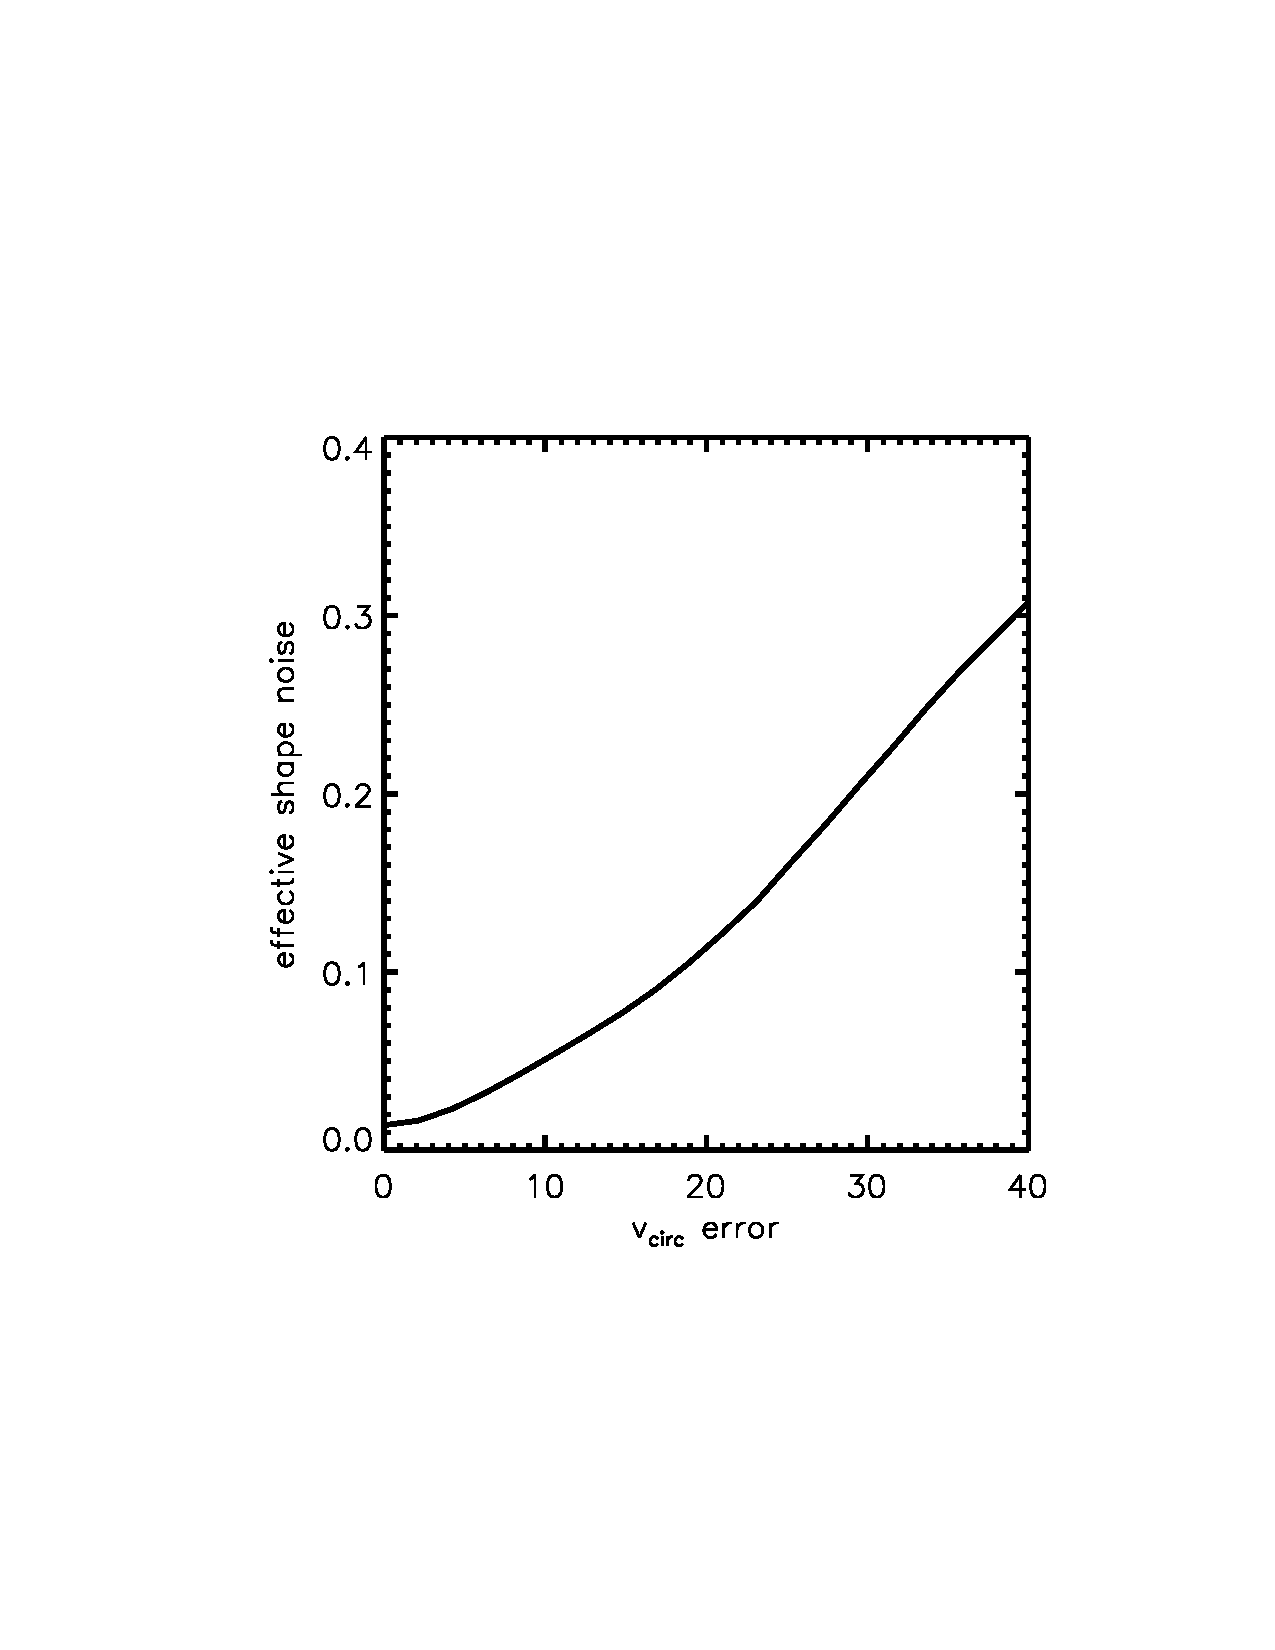
\includegraphics[width=0.45\linewidth, bb= 150 150 550 650,clip]{Plots/vcirc_error.pdf}
\caption{\footnotesize Effective shape noise $\sigma_{TF}$ as a  function of the
  measurement error on the disk circular velocity.}
\label{fig:shapeNoise}
\end{figure}


\begin{figure}[t]
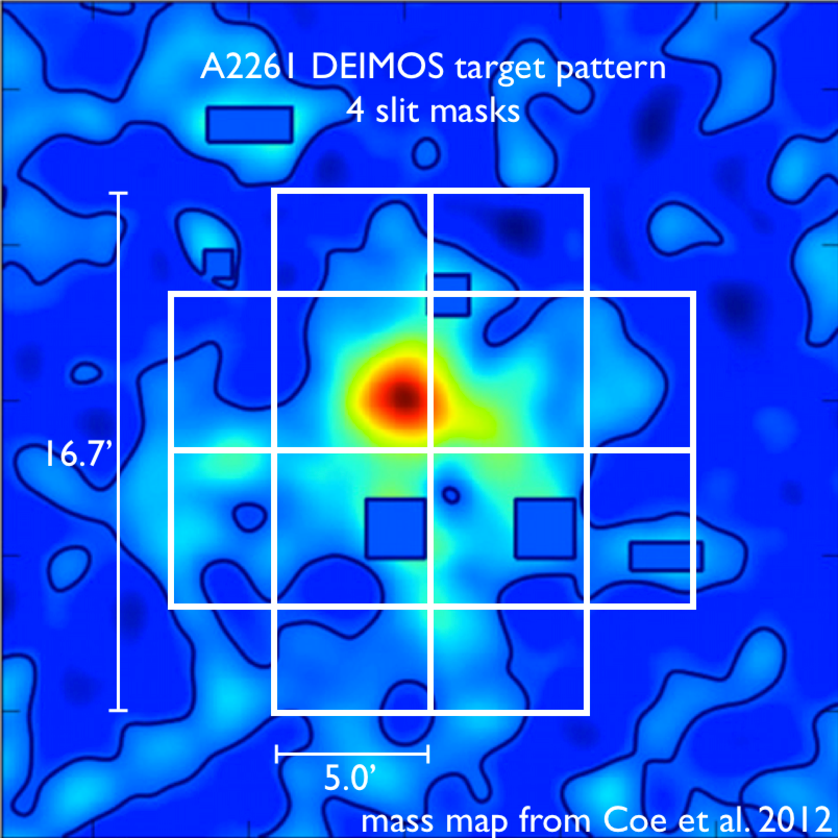
\includegraphics[width=0.45\linewidth]{Plots/a2261_deimos_mask.pdf}
\caption{\footnotesize Mass map of A2261 , with proposed DEIMOS slitmask geometry superposed.}
\label{fig:maskoverlay}
\end{figure}



\section{Technical Remarks}

\subsection{Targets and Exposures}

Abell 2261 ($z=0.225$, \citealt{Coe2012}) is an ideal target for testing this novel mass mapping technique since its high mass ($M_{\rm vir}\approx 2.2 \times 10^{15}\,M_{\odot}$) and moderate redshift produces a large lensing signal for background galaxies at $z\sim0.6-1.2$, and its angular size $R_{\rm vir} \approx 3\,{\rm Mpc} = 13.4'$ is well-matched to the DEIMOS field of view. We propose to cover this cluster with 4 slit masks, with most of the area covered twice by perpendicular masks to allow repeat observations of targets with $\Delta P.A.=90\degr$ (Figure~\ref{fig:maskoverlay}). This will enable us to measure velocities along both photometric axes to better constrain the shear.

Abell 2261 is part of the CLASH sample \citep{Postman2012} which obtained multi-wavelength HST data for the inner $\sim3'$ and has existing Subaru data in B, V, and R bands. We will target galaxies behind the cluster using a color selection modeled on the DEEP2 survey \citep{Newman2013} which successfully identified a large sample of high redshift galaxies and measured rotation curves using the [OII] emission line. To resolve the [OII] doublet, we will use the 1200 line/mm grating. The line flux needed for measuring kinematics with the DEIMOS configuration used by DEEP2 is $\gtrsim10^{-17}\,{\rm erg/s/cm^2}$ \citep{Kassin2012}. Using COSMOS data \citep{Jouvel2009}, we find that a BVR color selection of resolved ($r_{1/2}>0.5"$) galaxies from Subaru photometry with a target density of $1.5-2\,{\rm arcmin^{-2}}$ can efficiently select objects at $z\sim0.6-1.2$ with [OII] fluxes above this threshold. This strategy should produce a sample of $>100$ galaxies with two-dimensional kinematics measured at $z_{\rm}\approx0.8$. To ensure sufficient ${\rm S/N}$ in velocity measurements along both axes, we request \textbf{2 hour exposures $\times$ 4 masks = 8 hours shutter time}. [Morphology cuts?]


\subsection{Backup Program}

\subsection{Supplementary Observations}

\subsection{Status of Previously Approved Keck Programs}



\textcolor{Red}{The following sections are optional but highly recommended}
\subsection{Path to Science from Observations}

\subsection{Technical Concerns}

\subsection{Experience and Publications}

The team has extensive experience with optical spectroscopy including development of the spectroscopic pipeline used for SDSS and BOSS which have been applied to numerous extragalactic studies including measurement of the local Tully-Fisher relation. We have also led analyses of DEIMOS spectra as part of the DEEP2 survey, as well as weak lensing studies including shape measurement and the use of observables beyond shear. An abbreviated reference list follows, with papers using Lick or Keck data highlighted with an asterisk.

\begin{description}
\item \textit{Optical spectroscopy and Tully-Fisher analysis:}
  \begin{description}
  \item \** {Mostek}, N., {Coil}, A.~L., {Cooper}, M., {Davis}, M., {Newman}, J.~A., \&
    {Weiner}, B.~J. 2013, ApJ, 767, 89
  \item \** {Mostek}, N., {Coil}, A.~L., {Moustakas}, J., {Salim}, S., \& {Weiner}, B.~J.
    2012, ApJ, 746, 124
  \item {Schlegel}, D., {White}, M., \& {Eisenstein}, D. 2009, in Astronomy, Vol. 2010,
    astro2010: The Astronomy and Astrophysics Decadal Survey, 314
  \item \** {Schlegel}, D.~J. 1995, PhD thesis, UNIVERSITY OF CALIFORNIA, BERKELEY.
  \end{description}
\item \textit{Weak lensing shape measurement and analysis:}
  \begin{description}
  \item {George}, M.~R., {et~al.} 2012, ApJ, 757, 2
  \item {Huff}, E.~M., {Eifler}, T., {Hirata}, C.~M., {Mandelbaum}, R., {Schlegel}, D.,
    \& {Seljak}, U. 2011{\natexlab{a}}, ArXiv e-prints
  \item {Huff}, E.~M., \& {Graves}, G.~J. 2011, ArXiv e-prints
  \item {Huff}, E.~M., {Hirata}, C.~M., {Mandelbaum}, R., {Schlegel}, D., {Seljak}, U.,
    \& {Lupton}, R.~H. 2011{\natexlab{b}}, ArXiv e-prints
  \item {Melchior}, P., {Sutter}, P.~M., {Sheldon}, E.~S., {Krause}, E., \& {Wandelt},
    B.~D. 2013, ArXiv e-prints
  \item {Melchior}, P., {Viola}, M., {Sch{\"a}fer}, B.~M., \& {Bartelmann}, M. 2011,
    MNRAS, 412, 1552
  \end{description}
\end{description}

\subsection{Resources and Publication Timescale}

\renewcommand{\bibfont}{\footnotesize}
\begin{spacing}{0.}
\bibliographystyle{apj}
\bibliography{proposal}
\end{spacing}

\end{document}